\chapter{Results}
Several candidate satellites was studied before arriving at the combination of datasets presented here. Spatiotemporal consistency and resolution was given high priority. 
% when choosing a dataset.
The variable cloud mask is provided by many satellites. Providing valuable information in itself, but also for the retrieval of other variables restricted to cloud free conditions. Humidity's is a good example of such a variable.  The satellite product chosen for this project is the \acrfull{msg}. This is satellite is in geostationary orbit, has a exceptional temporal resolution. Knowing that the average lifetime of a cloud is 60min or less, it seems like a reasonable choice. \textbf{kilde Lohmann s.19} The finished dataset is named \acrfull{ecc}.

\section{Dataset - European Cloud Cover }
This section presents the developed algorithms necessary for the compilation of the dataset European Cloud Cover, ECC. It is pieces together from two sources, ERA5 reanalysis and METeosat second generation cloud mask. % This requires the regridding of one of them.

\acrfull{ecc} comprises of five variables collected from two sources; ERA5 and EUMETSAT. Preserving the resolution available in ERA5, while remapping the cloud mask to cloud fractions. The final product consist of the variables temperature, pressure, cloud fraction, specific and relative humidity. Hourly data on a $0.25^o$ uniform grid resolution in the period from April 2004 to December 2018. Total cloud cover is produced from area weighting cloud masks. This computations are described in \ref{sec:remapping}. The others are on their original format as provided by \acrfull{ecmwf}. A summary of the original sources of the dataset is given in table \ref{tab:dataset_summary}. More details on ERA5 is available in Section \ref{sec:era5} and see section \ref{sec:EUMETSAT_cloud_mask} for more information about cloud mask. 
\begin{table}[]
    \centering
    \resizebox{\textwidth}{!}{%
\begin{tabular}{c|c|c|c|c|}
\cline{2-5}
\multirow{4}{*}{}                                 & \multicolumn{2}{c|}{\textbf{ERA5}}                                                                                                   & \multicolumn{2}{c|}{\textbf{MSG2}}                                                                                                                \\ \cline{2-5} 
                                                  & \textbf{Type}                     & \textbf{Variables}                                                                               & \textbf{Type}                                                               & \textbf{Variables}                                                  \\ \cline{2-5} 
                                                  & Surface                           & \begin{tabular}[c]{@{}c@{}}2m Temperature\\ Surface pressure\end{tabular}                        & \multirow{2}{*}{Satelite retrival}                                          & \multirow{2}{*}{Cloud Mask}                                         \\ \cline{2-3}
                                                  & 1000 hPa                          & \begin{tabular}[c]{@{}c@{}}Relative Humidity\\ Specific Humidity\end{tabular}                    &                                                                             &                                                                     \\ \hline
\multicolumn{1}{|c|}{\textbf{Projection}}         & \multicolumn{2}{c|}{Uniform grid}                                                                                                    & \multicolumn{2}{c|}{Curve linear grid}                                                                                                            \\ \hline
\multicolumn{1}{|l|}{\textbf{Spatial resolution}} & \multicolumn{2}{c|}{$0.25^o$}                                                                                                        & \multicolumn{2}{c|}{-}                                                                                                                            \\ \hline
\multicolumn{1}{|c|}{\textbf{Output Frequencey}}  & \multicolumn{2}{c|}{Hourly}                                                                                                          & \multicolumn{2}{c|}{15 min}                                                                                                                       \\ \hline
\multicolumn{1}{|c|}{\textbf{Availability}}       & \multicolumn{2}{c|}{\begin{tabular}[c]{@{}c@{}}1979-onwards\\ Expected to be available from \\ 1950 some time in 2020.\end{tabular}} & \multicolumn{2}{c|}{2004-onward}                                                                                                                 \\ \hline
\multicolumn{1}{|c|}{\textbf{License}}           & \multicolumn{2}{c|}{\begin{tabular}[c]{@{}c@{}}Open Access. Need user \\ from Copernicus Data Storage.\end{tabular}}                  & \multicolumn{2}{c|}{\begin{tabular}[c]{@{}c@{}}Researcher Licences\\ to get 15min resolution.\\ Open access at \\ hourly resolution\end{tabular}} \\ \hline
\end{tabular}
}
\caption{Data description on the data present in the dataset ECC (European Cloud Cover). \textbf{Add projection as a column, Availability for download and the period of data.} There is a lot of work in combining the two datasets and processing it.}
\label{tab:dataset_summary}

\end{table}

\subsection{Domain}
For this project the geographical domain has been restricted latitude $\in[30,50]$ and longitude $\in [-15, 25]$. The resulting dimensions of the grid becomes $81\times161$ pixels. Argue that this area should be sufficient ot prove a concept. Seems like a reasonable start, to prove a concept. Figure \ref{fig:map} shows the region of Europe included in this dataset. Covering the Mediterranean areas.

\begin{figure}[h]
    \centering
    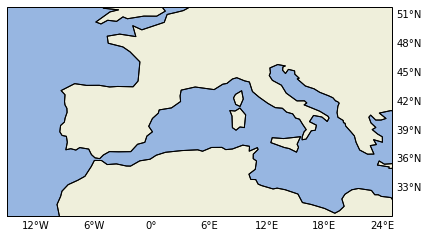
\includegraphics[scale = 0.7]{Chapter4_Results/figurs/Domain.png}
    \caption[Map over domain.]{Map showing the domain. The region covers southern Europe and northern Africa. The projection is the same as ECC (Plate Caree).}
    \label{fig:map}
\end{figure}

\begin{figure}
    \centering
    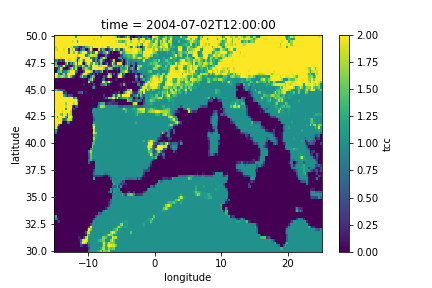
\includegraphics{Chapter4_Results/figurs/regridded_raw_satelite_image_to_make_sure_its_correcxt_area.png}
    \caption{Making sure its the correct area.}
    \label{fig:correct_area}
\end{figure}

\subsection{Physical basis of variable decision} \label{sec:ecc}
%%%%%%%%%%%%%%%%%%%%%%%%%%%%%%%%%%%%%%%%%%%%%%%%%%%%
%\subsubsection{Physical basis of variable decision} \label{sec:physical_basis}
The overall goal is to investigate if its enough information to predict cloud cover in the meteorological variables such as temperature, pressure and humidity. As discussed in Section \ref{sec:cloud_in_climate_system}, cloud dynamics is far more complicated than what can be describes by these variables. Not feasible in the foreseeable future to incorporate all the effects of micro-physics at a sufficient accuracy. Focusing on the macro-physical aspect of clouds its is reasonable to chose large scale variables.  Variables provided by a reliable estimate using reanalysis and other climate model. Ensuring that it is possible to build usable application of this in the future.

%As described in section \ref{sec:param_clouds} clouds are parameterised in many different ways using many different tools. Researchers have to this day not been able to incorporate the effects of clouds. 
\textbf{We hypothesise,} there is enough information in these variables to make a adaquate representation of cloud fraction. The following variables have been chosen because they are reliable (temperature and pressure) and/or cause the are essential in cloud formation (humidities). Other information may be present implicitly in these variables. It is worth noting that they are either surface variables or from the pressure level closest to the surface. All variables are produced by ERA5. This section will give a brief introduction to their role in cloud formation. 

From the weather maps on the news, low and high pressure systems might be familiar terms. Low pressure systems are often associated with precipitation, while high pressure systems are with nice weather. Due to its spherical geometry the earth is not equally heated. Warmer air rises, this generates a low pressure at the surface. As the air rises the temperature decreases. Colder air can retain less vapour, achieving saturation. Under supersaturated conditions some of this vapour condenses, generating cloud water, forming a cloud, and occasionally cloud precipitate. \textbf{This is often referred to as convection motion, and is typically associated with cumulus type clouds}. In presence of water, evaporation rates are also higher in a warmer climate. 

The earth system strives to be in balance. In areas of lower pressure the surrounding air flow toward the low pressure centre in order to offset the pressure difference. Due to the earth rotation and the Coriolis effect. \textit{Winds of a low pressure system swirl counterclockwise north of the equator and clockwise south of the equator.} In a high pressures system the air flows from the centre. \textit{Air from higher in the atmosphere sinks down to fill the space left as air is blown outward.} Winds transports the substances suspended in air, air pollution and humidity.

The dataset include both relative and specific humidity. Relative humidity is a measure of how much vapour the air contains, relative to much it can hold at that temperature. Its unitless, and it values ranges from $\left[ 0, 1 \right]$.  Conditions where relative humidity exceeds one are called supersaturated. Specific humidity ratio between mass of vapour and mass of air. Unit is $kg kg^{-1}$. \textbf{kilde s. 53, 54 Lohmann}. Whether the relative or specific humidity is the better predictor is not clear a priori. The data is gathered from the model level closest to the surface, at an altitude of 1000hPa. \textbf{kilde Lohmann s. 81-84}

\subsection{Computing cloud fractions (ny overskrift == preprocessing?)} \label{sec:remapping}
\begin{figure}
    \centering
    
    
\tdplotsetmaincoords{60}{110}
%
\pgfmathsetmacro{\rvec}{1.0}
\pgfmathsetmacro{\thetavec}{30}
\pgfmathsetmacro{\phivec}{60}

\pgfmathsetmacro{\deltathetavec}{40}
\pgfmathsetmacro{\deltaphivec}{80}

%
\begin{tikzpicture}[scale=5,tdplot_main_coords]
    \coordinate (O) at (0,0,0); % origo

    \coordinate (z) at (0, 0, 1.0); % origo
    %\draw[thin, <->] (1, 0.7, 1.16) -- (1, 0.52, 1.2) node[pos = 0.8, above right]{\Large $d\theta$};
    
    \draw[very thick,->] (0,0,0) -- (1.7, 0, 0) node[anchor=north east]{\Large $x$};
    \draw[very thick,->] (0,0,0) -- (0, 1.7, 0) node[anchor=north west]{\Large $y$};
    \draw[very thick,->] (0,0,0) -- (0, 0, 1.7) node[anchor=south]{\Large $z$};
    \shade[ball color = teal, opacity = 0.1] (0,0,0) circle [radius=\rvec];
    \draw (0,0,0) circle [radius=\rvec];
    
    \tdplotsetcoord{P}{\rvec}{\thetavec}{\phivec}
    \tdplotsetcoord{dP}{\rvec}{\deltathetavec}{\phivec}
    
    \tdplotsetcoord{G}{\rvec}{\thetavec}{\deltaphivec}
    \tdplotsetcoord{dG}{\rvec}{\deltathetavec}{\deltaphivec}

    \draw[very thick, color=teal, opacity = 0.3] (O) -- (G) node[above right]  {};
    \draw[very thick, color=teal, opacity = 0.6] (O) -- (dG) node[above right] {};    
    \draw[very thick, color=teal, opacity = 0.6] (O) -- (P) node[above right]  {};
    \draw[very thick, color=teal, opacity = 0.6] (O) -- (dP) node[above right] {};
    
    \draw[dashed, color=teal] (O) -- (Pxy);
    \draw[dashed, color=teal] (dP) -- (Pxy);
    %\draw[dashed, color=red] (Pz) -- (Py);


    %\draw[dashed, color=red] (dP) -- (Pxy);
    
    \draw[dashed, color=teal] (O) -- (Gxy);
    \draw[dashed, color=teal] (dG) -- (Gxy);
    \draw[dashed, color=black,looseness = 10, bend left] (z) -- (G)  node[pos = 0.6, above right] {\Large $rsin\theta$};
    \draw[dashed, color=teal,looseness = 10, bend left] (z) -- (G);
    \draw[dashed, color=teal, bend right] (P) -- (z);
    
    
    \draw [] (\phivec:0.5)  arc (\phivec:\deltaphivec:0.5) node [below right, pos=0.3] {\Large $d\phi$};

    
    %\tdplotdrawarc[tdplot_rotated_coords, ->]{(dP)}{.7}{(Pxy)}
    
    \draw[dashed, very thick, color=teal, fill = teal, opacity = 0.2] (P) -- (dP) -- (dG) -- (G) -- (P);
    \draw[dashed, very thick, color=teal] (P) -- (dP) -- (dG) -- (G) -- (P);
    \draw[dashed, color=black] (dG) -- (G) node[pos = 0.5, above right] {\Large $rd\theta$};
    \draw[dashed, color=teal] (dG) -- (G);    \tdplotdrawarc[]{(O)}{0.4}{0}{\phivec}{anchor=north}{\Large $\phi$}
    %\tdplotdrawarc{(O)}{0.2}{0}{\deltathetavec}{anchor=north}{$\theta$}

    \tdplotsetthetaplanecoords{\phivec};
    
    \tdplotdrawarc[tdplot_rotated_coords]{(0,0,0)}{0.8}{0}%
        {\thetavec}{anchor=south west}{\Large $\theta$};
    
    \tdplotdrawarc[tdplot_rotated_coords, pos = 0.5]{(0,0,0.2)}{0.26}{0}%
        {\thetavec}{anchor = south west,shift={(4mm,-5mm)}}{\Large $d\theta$};
        
    %\tdplotdrawarc[tdplot_rotated_coords, <->]{(0.1, 0.2, 0)}{.5}{0}{\thetavec}{anchor=east}{\Large $d\theta$}
    \shade[ball color=teal,tdplot_screen_coords,opacity=0.1] (O) circle[radius=\rvec];
    \foreach \X/\Y in {xy/z,yz/x,zx/y}
        {\begin{scope}[canvas is \X\space plane at \Y=\rvec]
         \fill circle[radius=1pt];
        \end{scope}}
    \end{tikzpicture}
    
    \caption[Square projected in spherical coordinates]{Properties of a square in spherical coordinates. This is used in the area weighted remapping scheme. Theta er vell også missvisende. Her er den degrees south? \textbf{Trenger figuren subscripts med i og j.}}
    \label{fig:spherical_coords}
\end{figure}
\tdplotsetmaincoords{60}{110}
%
\pgfmathsetmacro{\rvec}{1.6}
\pgfmathsetmacro{\thetavec}{30}
\pgfmathsetmacro{\phivec}{60}

\pgfmathsetmacro{\deltathetavec}{40}
\pgfmathsetmacro{\deltaphivec}{80}

\begin{figure}
    \centering
    
    
\tdplotsetmaincoords{60}{110}
%
\pgfmathsetmacro{\rvec}{1.0}

\pgfmathsetmacro{\thetavec}{30}
\pgfmathsetmacro{\deltathetavec}{40}
\pgfmathsetmacro{\deltatwothetavec}{50}
\pgfmathsetmacro{\deltathreethetavec}{60}

\pgfmathsetmacro{\phivec}{-30}
\pgfmathsetmacro{\deltaphivec}{10}
\pgfmathsetmacro{\deltatwophivec}{50}
\pgfmathsetmacro{\deltathreephivec}{90}

\begin{tikzpicture}[scale=5,tdplot_main_coords]

    %%%%%%%%%%%%%% Setting up axis and coordinate system.
    \coordinate (O) at (0,0,0); % origo
    \coordinate (z) at (0, 0, \rvec); % origo
    %\draw[thin, <->] (1, 0.7, 1.16) -- (1, 0.52, 1.2) node[pos = 0.8, above right]{\Large $d\theta$};
    \draw[very thick,->, opacity = 1.] (0,0,0) -- (1.7, 0, 0) node[anchor=north east]{\Large $x$};
    \draw[very thick,->,  opacity = 1.] (0,0,0) -- (0, 1.7, 0) node[anchor=north west]{\Large $y$};
    \draw[very thick,->,  opacity = 1.] (0,0,0) -- (0, 0, 1.7) node[anchor=south]{\Large $z$};
    \shade[ball color = teal, opacity = 0.1] (0,0,0) circle [radius=\rvec];
    \draw (0,0,0) circle [radius=\rvec];

    %%%%%%%%%%%%%%%%%%%%%%%%%%%% first column
    \tdplotsetcoord{P}{\rvec}{\thetavec}{\phivec}
    \tdplotsetcoord{dP}{\rvec}{\deltathetavec}{\phivec}
    \tdplotsetcoord{G}{\rvec}{\thetavec}{\deltaphivec}
    \tdplotsetcoord{dG}{\rvec}{\deltathetavec}{\deltaphivec}
    
    \draw[dashed, very thick, color=teal, fill = teal, opacity = 0.2] (P) -- (dP) -- (dG) -- (G) -- (P);
    \draw[dashed, very thick, color=teal] (P) -- (dP) -- (dG) -- (G) -- (P);
    
    \tdplotsetcoord{a}{\rvec}{\deltathetavec}{\phivec}
    \tdplotsetcoord{b}{\rvec}{\deltatwothetavec}{\phivec}
    \tdplotsetcoord{c}{\rvec}{\deltathetavec}{\deltaphivec}
    \tdplotsetcoord{d}{\rvec}{\deltatwothetavec}{\deltaphivec}
    
    \draw[dashed, very thick, color=teal, fill = teal, opacity = 0.2] (a) -- (b) -- (d)-- (c) -- (a);
    \draw[dashed, very thick, color=teal] (a) -- (b) -- (d)-- (c) -- (a);
    
    \tdplotsetcoord{e}{\rvec}{\deltatwothetavec}{\phivec}
    \tdplotsetcoord{f}{\rvec}{\deltathreethetavec}{\phivec}
    \tdplotsetcoord{g}{\rvec}{\deltatwothetavec}{\deltaphivec}
    \tdplotsetcoord{h}{\rvec}{\deltathreethetavec}{\deltaphivec}
    
    \draw[dashed, very thick, color=teal, fill = teal, opacity = 0.2] (e) -- (f) -- (h)-- (g) -- (e);
    \draw[dashed, very thick, color=teal] (e) -- (f) -- (h)-- (g) -- (e);

    %%%%%%%%%%%%%%%%%%%%%%%%%%%%%%%% second column
      
    \tdplotsetcoord{P}{\rvec}{\thetavec}{\deltaphivec}
    \tdplotsetcoord{dP}{\rvec}{\deltathetavec}{\deltaphivec}
    \tdplotsetcoord{G}{\rvec}{\thetavec}{\deltatwophivec}
    \tdplotsetcoord{dG}{\rvec}{\deltathetavec}{\deltatwophivec}
    
    \draw[dashed, very thick, color=teal, fill = teal, opacity = 0.2] (P) -- (dP) -- (dG) -- (G) -- (P);
    \draw[dashed, very thick, color=teal] (P) -- (dP) -- (dG) -- (G) -- (P);
  
      
    \tdplotsetcoord{a}{\rvec}{\deltathetavec}{\deltaphivec}
    \tdplotsetcoord{b}{\rvec}{\deltatwothetavec}{\deltaphivec}
    \tdplotsetcoord{c}{\rvec}{\deltathetavec}{\deltatwophivec}
    \tdplotsetcoord{d}{\rvec}{\deltatwothetavec}{\deltatwophivec}
    
    \draw[dashed, very thick, color=teal, fill = teal, opacity = 0.2] (a) -- (b) -- (d)-- (c) -- (a);
    \draw[dashed, very thick, color=teal] (a) -- (b) -- (d)-- (c) -- (a);
  
  
    \tdplotsetcoord{e}{\rvec}{\deltatwothetavec}{\deltaphivec}
    \tdplotsetcoord{f}{\rvec}{\deltathreethetavec}{\deltaphivec}
    \tdplotsetcoord{g}{\rvec}{\deltatwothetavec}{\deltatwophivec}
    \tdplotsetcoord{h}{\rvec}{\deltathreethetavec}{\deltatwophivec}
    
    \draw[dashed, very thick, color=teal, fill = teal, opacity = 0.2] (e) -- (f) -- (h)-- (g) -- (e);
    \draw[dashed, very thick, color=teal] (e) -- (f) -- (h)-- (g) -- (e);
    
    
    %%%%%%%%%%%%%%%%%%%%%%%%%%%%%%%% third column
    \tdplotsetcoord{P}{\rvec}{\thetavec}{\deltatwophivec}
    \tdplotsetcoord{dP}{\rvec}{\deltathetavec}{\deltatwophivec}
    \tdplotsetcoord{G}{\rvec}{\thetavec}{\deltathreephivec}
    \tdplotsetcoord{dG}{\rvec}{\deltathetavec}{\deltathreephivec}
    
    \draw[dashed, very thick, color=teal, fill = teal, opacity = 0.2] (P) -- (dP) -- (dG) -- (G) -- (P);
    \draw[dashed, very thick, color=teal] (P) -- (dP) -- (dG) -- (G) -- (P);
  
    \tdplotsetcoord{a}{\rvec}{\deltathetavec}{\deltatwophivec}
    \tdplotsetcoord{b}{\rvec}{\deltatwothetavec}{\deltatwophivec}
    \tdplotsetcoord{c}{\rvec}{\deltathetavec}{\deltathreephivec}
    \tdplotsetcoord{d}{\rvec}{\deltatwothetavec}{\deltathreephivec}
    
    \draw[dashed, very thick, color=teal, fill = teal, opacity = 0.2] (a) -- (b) -- (d)-- (c) -- (a);
    \draw[dashed, very thick, color=teal] (a) -- (b) -- (d)-- (c) -- (a);
  
    \tdplotsetcoord{e}{\rvec}{\deltatwothetavec}{\deltatwophivec}
    \tdplotsetcoord{f}{\rvec}{\deltathreethetavec}{\deltatwophivec}
    \tdplotsetcoord{g}{\rvec}{\deltatwothetavec}{\deltathreephivec}
    \tdplotsetcoord{h}{\rvec}{\deltathreethetavec}{\deltathreephivec}
    
    \draw[dashed, very thick, color=teal, fill = teal, opacity = 0.2] (e) -- (f) -- (h)-- (g) -- (e);
    \draw[dashed, very thick, color=teal] (e) -- (f) -- (h)-- (g) -- (e);
    
    %%%%%%%%%%%%%%%%%%%%%%%%%% Adding coordinate information

    % First column
    \draw[thick](0.3, -0.25, 0.5)node[scale=0.8, rotate = -15]{$(i,j-1)$};
    \draw[thick](0.3, -0.17, 0.7)node[scale=0.8, rotate = -15]{$(i+1,j-1)$};
    \draw[thick](0.3, -0.3, 0.3)node[scale=0.8, rotate = -15]{$(i-1,j-1)$};

    % Second column
    \draw[thick](0.5, 0.3, 0.65)node[scale=0.8, rotate = 5]{$(i,j)$};
    \draw[thick](0.5, 0.3, 0.85)node[scale=0.8, rotate = 5]{$(i+1,j)$};
    \draw[thick](0.5, 0.3, 0.45)node[scale=0.8, rotate = 5]{$(i-1,j)$};
    
    % Third column
    \draw[thick](0.5, 0.73, 0.87)node[scale=0.8, rotate = 35]{$(i,j+1)$};
    \draw[thick](0.5, 0.8, 0.7)node[scale=0.8, rotate = 35]{$(i-1,j+1)$};

    \draw[thick](0.05, 0.45, 0.73)node[scale=0.8, rotate = 35]{$(i+1,j+1)$};

    \tdplotsetthetaplanecoords{\phivec};
    \shade[ball color=teal,tdplot_screen_coords,opacity=0.1] (O) circle[radius=\rvec];
    \foreach \X/\Y in {xy/z,yz/x,zx/y}
        {\begin{scope}[canvas is \X\space plane at \Y=\rvec]
         \fill circle[radius=1pt];
        \end{scope}}
    \end{tikzpicture}
    
    \caption{Sketch to illustrated the relative size of neighbouring pixels in uniform grid of ECC, projected onto spherical coordinates. The areas of pixels in a uniform grid decrease poleward.}
    \label{fig:relative_size_neigbouring_pixels}
\end{figure} % move
Computing cloud fractions based on cloud mask requires a regridding scheme, such as mean, nearest neighbour or area weighted. For this particular task the area weighted seemed most appropriate. This section will provided a step-by-step walk-though of the necessary preprocessing done for the compilation of ECC. Transforming clouds masks provided in \textit{space-view} to cloud fractions on a uniform grid. EUMETSAT doesn't provide suitable software to tackle this particular task (personal communication EUMETSAT staff). Building the dataset requires the implementations of this software.

%In order to build the dataset to cover our needs for this application, the area weighting and regridding to ERA5 grid was implemented in Python.
%\textit{The regridding functionality was implemented in Python and is publicly available though the project GitHub. Running the code for all year takes a while on a regular computer. Each time step is stored in individual grib-files. One netCDF-file is stored for its coordinate-information. Its done like this because of storage limitations. One netCDF-file take up roughly 1GB of memory. }
\textbf{Write summary based on this list to introduce section.}
\begin{enumerate}
    \item Utlede ligningene for areal
    \item Area of a square in spherical coordinates
    \item Estimating the changes in latitude and longitude. Based on information about the centre of the pixels. 
    \item Contributions from boundaries and corners. 
    \item Validating the algorithm against cdo compute areas and the focusing on the artefact. Making short videos of 500 frames to look at the evolution of cloud cover, to double check that it looks reasonable. 
    \item Cause of many errors, the data is flipped depending on the file-format it is provided in shuffled/reversed (opp ned, bak fram). Similar shape of distribution of cloud cover as other satelite,usnnhetstegn mens skyfracsjon er en stor funksjon av 
    item \textbf{Obs Obs - gridtype space view}
    \item Has anyone managed to handle this kind of data? Obviously the space view perspective grid is natural choice for products derived from geostationary platforms and thus standard in EUMETSAT. 
    \item Bytt curvelinear til space view.
    \item Latitude (degrees north), Longitude degrees east.
\end{enumerate}

Implementing this algorithm requires deriving the equation necessary for computing the area weighting and detection of pixels contributing to the particular cells in the other coordinate system. The satellite retrievals are provided in a \textit{space-view} grid. Pixel-areas are computed using spherical coordinates. Deriving the equation for computing the area of an square in spherical coordinates, requires integrating over changes in latitude and longitude. The general expression for the area of a square in spherical coordinates, is given by the following integral. 
\begin{equation} \label{eq:sphere_integral}
    A = -R^2\int_{ \theta - \delta \theta }^{\theta + \delta \theta} \int_{ \phi - \delta \phi }^{\phi + \delta \phi} cos\left( \theta' \right) d\phi' d\theta'
\end{equation}
This can be rewriting into, \textbf{add indices $(i, j)$ ..?}
\begin{equation} \label{eq:sphere_finish}
    A \left( \theta, \phi, \delta \theta, \delta \phi   \right)= 2R^2 \left( sin\left( \theta + \delta \theta  \right) - sin\left(  \theta - \delta \theta  \right) \right) \delta \phi
\end{equation}
Relating this to Figure \ref{fig:spherical_coords} $d \theta = 2 \delta \theta$, $d \phi = 2 \delta \phi$. Figure \ref{fig:spherical_coords} shows a square projected onto a sphere. Highlighting the parts necessary to compute a area. \textbf{Update this based on how the equations are solved.} Here R denotes the distance to earth centre, $\theta$ the latitude and $\phi$ the longitude. The latitude and the extend of the pixel is terms in this equation. Equation \ref{eq:sphere_finish} is implemented. 

% Estimating the extent of the cell.
The coordinate information is provided as the latitude, $\theta$ (degrees north) and longitude, $\phi$ (degrees east) of the centre of the pixel. The areas computation require information about the extent of the cell, this requires some simplifications. The changes on longitude (latitude) at a certain pixel are estimated by the average distance to neighbouring points in the horizontal (vertical). Approximation of $d\phi$ and $d\theta$ have been done based on the two-dimensional fields of latitude and longitude values according to the below equations, \eqref{eq:app_lon} and  \eqref{eq:app_lat}. Figure \ref{fig:estimate_dlat_dlon} illustrates how neighbouring pixels, of same extent, appear in spherical coordinates. The area decreases poleward. 
% The below approach underestimates the extent a bit? Jeg tror ikke det .. 
Let the horizontal extent of a pixel $(i,j)$ be determined by the the averaged distance between the longitude of neighbouring pixels, see Equation \eqref{eg:app_lon}. The same follows for the vertical extent, but in Equation \eqref{eq:app_lat} it is dependant of the latitude values. 

\tdplotsetmaincoords{60}{110}
%
\pgfmathsetmacro{\rvec}{1.6}
\pgfmathsetmacro{\thetavec}{30}
\pgfmathsetmacro{\phivec}{60}

\pgfmathsetmacro{\deltathetavec}{40}
\pgfmathsetmacro{\deltaphivec}{80}

\begin{figure}
    \centering
    
    
\tdplotsetmaincoords{60}{110}
%
\pgfmathsetmacro{\rvec}{1.0}

\pgfmathsetmacro{\thetavec}{30}
\pgfmathsetmacro{\deltathetavec}{40}
\pgfmathsetmacro{\deltatwothetavec}{50}
\pgfmathsetmacro{\deltathreethetavec}{60}

\pgfmathsetmacro{\phivec}{-30}
\pgfmathsetmacro{\deltaphivec}{10}
\pgfmathsetmacro{\deltatwophivec}{50}
\pgfmathsetmacro{\deltathreephivec}{90}



\begin{tikzpicture}[scale=5,tdplot_main_coords, 
                    mycirc/.style={circle,fill=blue!20, minimum size=0.5cm}]

    %%%%%%%%%%%%%% Setting up axis and coordinate system.
    \coordinate (O) at (0,0,0); % origo
    \coordinate (z) at (0, 0, \rvec); % origo
    %\draw[thin, <->] (1, 0.7, 1.16) -- (1, 0.52, 1.2) node[pos = 0.8, above right]{\Large $d\theta$};
    \draw[very thick,->, opacity = 1.] (0,0,0) -- (1.7, 0, 0) node[anchor=north east]{\Large $x$};
    \draw[very thick,->,  opacity = 1.] (0,0,0) -- (0, 1.7, 0) node[anchor=north west]{\Large $y$};
    \draw[very thick,->,  opacity = 1.] (0,0,0) -- (0, 0, 1.7) node[anchor=south]{\Large $z$};
    \shade[ball color = teal, opacity = 0.1] (0,0,0) circle [radius=\rvec];
    \draw (0,0,0) circle [radius=\rvec];

    
    \tdplotsetcoord{a}{\rvec}{\deltathetavec}{\phivec}
    \tdplotsetcoord{b}{\rvec}{\deltatwothetavec}{\phivec}
    % Changeing the rightmost part 
    \tdplotsetcoord{c}{\rvec}{\deltathetavec-5}{\deltaphivec}
    \tdplotsetcoord{d}{\rvec}{\deltatwothetavec+5}{\deltaphivec}
    
    \draw[dashed, very thick, color=teal, fill = teal, opacity = 0.2] (a) -- (b) -- (d)-- (c) -- (a);
    \draw[dashed, very thick, color=teal] (a) -- (b) -- (d)-- (c) -- (a);

    \tdplotsetcoord{a}{\rvec}{\deltathetavec-5}{\deltaphivec}
    \tdplotsetcoord{b}{\rvec}{\deltatwothetavec+5}{\deltaphivec}
    \tdplotsetcoord{c}{\rvec}{\deltathetavec-10}{\deltatwophivec}
    \tdplotsetcoord{d}{\rvec}{\deltatwothetavec+10}{\deltatwophivec}
    
    \draw[dashed, very thick, color=teal, fill = teal, opacity = 0.2] (a) -- (b) -- (d)-- (c) -- (a);
    \draw[dashed, very thick, color=teal] (a) -- (b) -- (d)-- (c) -- (a);
        
    % First column
    %\node[draw] at (0, -2)  (c)     {C};
    %\node[draw] at (0.3, -0.25, 0.5) {$\phi_{(i,j-1)}$};
    %\node[draw, thick] at (0.5, 0.3, 0.65) {$\phi_{(i,j)})$};
    %\node[draw, thick] at (0.5, 0.73, 0.87) {$(i,j+1)$};
    \filldraw [teal, label=above:{$\phi_{(i,j-1)}$}]  (0.3, -0.25, 0.5) circle (1pt);
    \filldraw [teal, label=above:{$\phi_{(i,j-1)}$}]  (0.5, 0.3, 0.65)  circle (1pt);
    \filldraw [teal, label=above:{$\phi_{(i,j-1)}$}]  (0.5, 0.73, 0.87) circle (1pt);
    
    \tdplotsetcoord{a}{\rvec}{\deltathetavec-10}{\deltatwophivec}
    \tdplotsetcoord{b}{\rvec}{\deltatwothetavec+10}{\deltatwophivec}
    \tdplotsetcoord{c}{\rvec}{\deltathetavec-15}{\deltathreephivec}
    \tdplotsetcoord{d}{\rvec}{\deltatwothetavec+15}{\deltathreephivec}
    
    \draw[dashed, very thick, color=teal, fill = teal, opacity = 0.2] (a) -- (b) -- (d)-- (c) -- (a);
    \draw[dashed, very thick, color=teal] (a) -- (b) -- (d)-- (c) -- (a);
    
    \draw [decorate,decoration={brace, amplitude=12pt, mirror}, xshift=0pt, yshift=0pt]
    (0.3, -0.25, 0.1) -- (0.5, 0.83, 0.47) node [black,midway,xshift=0.2cm, yshift = -1.5cm, very thick] {\Large $\left| \phi_{i+1,j} - \phi_{i-1, j} \right| $};
    
    \draw [decorate,decoration={brace, amplitude=12pt}, xshift=0pt, yshift=0pt]
    (0.5, 0.3, 0.65) -- ((0.5, 0.5, 0.73) node [black,midway,xshift=0cm, yshift = 2.cm, very thick] {\Large $\delta \phi_{(i, j)}$};

    \tdplotsetthetaplanecoords{\phivec};
    \shade[ball color=teal,tdplot_screen_coords,opacity=0.1] (O) circle[radius=\rvec];
    \foreach \X/\Y in {xy/z,yz/x,zx/y}
        {\begin{scope}[canvas is \X\space plane at \Y=\rvec]
         \fill circle[radius=1pt];
        \end{scope}}
    \end{tikzpicture}
    
    \caption{Illustrating three neighbouring pixels on a sphere in the \textit{space-view} grid provided by EUMETSAT. Estimating the changes in longitude. Used to explain equation \eqref{eq:app_lon}. \textbf{Trude: Bør jeg ha lignende figure for latitude eller holder det å si det det finnes tilsvarende i vertikalen også.}}
    \label{fig:estimate_dlon}
\end{figure}

The cloud mask pixels are smallest at the nadir point, increasing in all other directions. Figure \ref{fig:estimate_dlon} shows a example of three neighbouring pixels where the apparent pixel size increase going eastward. This results in different distances to the right and left neighbour. Argue that the most robust estimate of the extent of the cell is made by averaging the distance to both neighbours. The is done in \eqref{eq:app_lon}. 

Failed to derive equations for trapezoidal shapes in spherical coordinate, therefore it never made sense to keep a different left, right, up and down extent. \textbf{Not sure how to include this}
%Since changes in degrees varies linearly this should not affect the extent of the cell. More than the error already present in the data. Det forklarer bare hvorfor buelengde ikke er nødvendig.
\begin{equation} \label{eq:app_lon}
    \delta \phi_{i,j} = \left| \frac{\phi_{i+1,j} - \phi_{i-1, j}}{4} \right|
\end{equation}
\begin{equation} \label{eq:app_lat}
    \delta \theta_{i,j} = \left| \frac{\theta_{i,j+1} - \theta_{i, j-1}}{4} \right|
\end{equation}

% Detecting which pixels that contribute to a cell.
Computing the area weighted average of cloud masks requires detecting the grid$_{\text{MGS}}$ contributing to the grid$_{\text{ERA5}}$ cell, and computing their area. The pixels are divided into five categories, centre, left, right, up and down boundary. 

Let the subscripts denote the dataset pertaining to a particular grid. Grid$_{\text{MGS}}$ refers to the space-view grid of the \acrlong{msg} and grid$_{\text{ECC}}$ refers to the uniform grid originating from ERA5. It is worth noting that the grid$_{\text{ECC}}$ would be the same as grid$_{\text{ECC}}$.
\begin{figure}
    \centering
    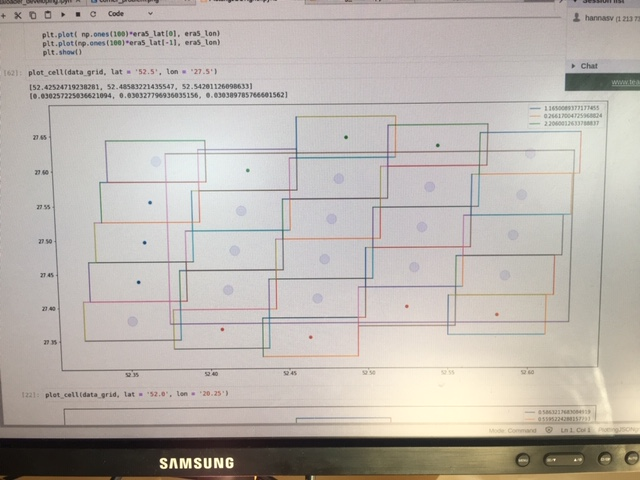
\includegraphics[scale = 0.6]{Chapter4_Results/figurs/remapping-pixels.JPG}
    \caption{Remapping one cell, studying the number of pixels contributing to a cell.}
    \label{fig:my_label}
\end{figure}

\begin{equation} \label{eq:tot_area}
    A = \sum_{i=0}^{N} a_i
\end{equation}

\begin{equation} \label{eq:area_weighting}
    CF_{ECC} = \frac{1}{A} \sum_{i=0}^{N} a_i m_i
\end{equation}

One can easily prove that if all the mask $m_i = 0$ the cloud fraction, $CF_{ECC}=1$. This would not be if the total area A, was determine by the extent of ERA5/ECC cell. This explains why the overlap of neighbouring cell is not a cause for concern. The cloud fractions will not give unphysical values. The only affect worth mentioning is that some cloud mask, located at boundary pixels, contribute a marginally more to the fraction than they should. Argue that this is o little importance in the big picture.
% For the boundary categories we only include the contribution from within the cell. This is not actually a strict condition, including the entire area would still keep the fraction within its normal bounds of 0 and 1. However the boundary pixels would have a larger effect on the mean cloud cover since they contribute to several pixels. The footprint size effect on the distribution of cloud cover. For a large pixel size, and less contributing pixels we expect a higher number of grid-cells with close to 0 or 1 cloud amount. Since it alter the number of components you compute the average from.

% The cells in grid$_{\text{MGS}}$ contributing to a particular cell in grid$_{\text{ERA5}i,j}$ is fixed. In order to save computations on areas and detecting contribution pixels these are saved to \acrshort{json}-files. Made available in the the GitHub repository for supplementary material \href{https://github.com/hannasv/MS-suppl}{https://github.com/hannasv/MS-suppl}.

% Since the grid is constant, this is only done once and their indices and computed areas are stored in  Java Script Object Notification, json-files in the GitHub repository for supplementary material.

The cloud masks are provided from EUMETSAT in multiple formats. The grib-format takes up less disk space. However this format doesn't provide coordinates for grid types such as space view. This information is available i \acrshort{netcdf}-format and is made available for the reader via the supplementary folder. All satellite images are provided using the same grid (personal correspondence with EUMETSAT staff). Occasionally both the standby and the operational scan at the same time. To reduce the perturbations due to parallax of cloud in the data the operational satellite is chosen, given the choice.

\subsection{ARTEFACT and LAND, SEA and Coastline masks} \label{sec:artefact}
The land sea masks are regridded from the HTAP-masks provided by \acrfull{metno}.  In its original format the HTAP masks have a $0.1^o$ resolution. Global coverage, not including the polar regions. These are re-gridded to a suitable resolution of $0.25^o$ using functionality available in PyAEROCOM (\href{https://pyaerocom.met.no/}{https://pyaerocom.met.no/}). A python toolbox the \acrfull{aerocom} project. Storing only the domain relevant, available in the project supplementary repository. 

\textbf{TODO:} Running the artefact filters to compute how many times this occurs. Make histogram.

Filters available is land, sea, coastline and artefact. The coastline is defined to be all pixel that is not 100\% either land or sea. For land pixels, coastline pixel exceeding a 50\% threshold is included, the other pixels are regarded at the sea. Argue that this is OK since this pixels at a level of at least 50\% is most like sufficiently affected by maritime conditions that its OK to classify them as sea pixels.

Some may want to argue that all pixels that are below 100\% coast probably is maritime conditions.

Defining the artefact according to equation, 
\begin{equation} \label{eq:artefact}
    \theta + \frac{1}{3}\phi < 40
\end{equation}
Figure \ref{fig:filter_artefact} show the artefact detecting filter. To keep memory-requirements to a minimum only the parts of the filters relevant domain is stored in the supplementary material for this project.

\begin{figure}
    \centering
    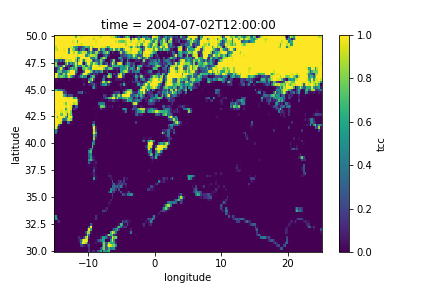
\includegraphics{Chapter4_Results/figurs/example_artefact.png}
    \caption[Artefact in European Cloud Cover dataset.]{Snapshop of artefact that is present in the dataset, ECC. The frequency of occurrence is currently unknown. \textbf{Plan to use the filter on every hour, storing the signal and plotting it in a histogram.}}
    \label{fig:example_artefact}
\end{figure}

\begin{figure*}[hp]
        \begin{subfigure}[b]{0.475\textwidth}
            \centering
            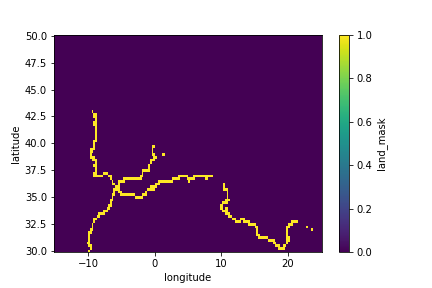
\includegraphics[scale=0.5]{Chapter4_Results/figurs/restricted_to_artefact.png}
            \caption[Filter activated to detect the region of Spain, Portugal and Northern Africa.]
            {{\small Filter activated to detect the region of Spain, Portugal and Northern Africa.}}
            \label{fig:filter_artefact}
        \end{subfigure}
        \hfill
        \begin{subfigure}[b]{0.475\textwidth}  
            \centering 
            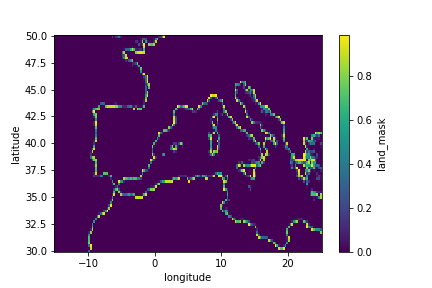
\includegraphics[scale=0.5]{Chapter4_Results/figurs/detecting_coast.png}
            \caption[]%
            {{\small Percentage of land in coastline pixels. }}    
            \label{fig:entire_coastline_detected}
        \end{subfigure}

        \caption[Different approaches for detecting the artefact, separating the land, sea and coastline pixels.]
        {\small Different approaches for detecting the artefact, separating the land, sea and coastline pixels. Filters to remove artefact in future. Can also use this compute statistics over land and ocean. Add land sea mask as subplot. }
        \label{fig:filters}
    \end{figure*}

Leaving the artefact in the data, its a thesis in itself to remove this without doing to much damage to the parts that are actually clouds that also produce a signal.

\subsection{Missing Data} \label{sec:missing_values}
As always when working with observations. The sensors fail to collect  measurements and data is missing. This can be either individual pixels or entire disks. Since the individual pixels are remapped to fractions by using the area weighted mean, NaN's don't appear too be an issue. When the entire disks are missing, the closest time step available within the previous and trailing 45 minutes are chosen. Gaps that not possible to fill in this way are documented in \textbf{X}. Manually generated datasets are prone to human error. The extra documentation is to ensure the user of what data is included and what is not. The missing values was double checked, but there might still be some data available online that is not included, however this amount should be small. Figure \ref{fig:heatmap_missing_values} show how many hours, that is missing from each of the month in the relevant time period. 

In some cases the data has been destroyed prior to archiving, and can never be recovered. The EUMETSAT staff has been made aware of this problem. The requested data has entered infinity loop without being detected by EUMETSAT along with max pending request restrictions (20), this has slowed things down in addition to create gaps in the data. One request can contain ca. 3.5 months of hourly data. After downloading the data the author had detect missing times and manually choose the closest time step available within the previous and trailing 45 minutes are chosen. Based on this experience the author would recommend that the the GUI or API's available for downloading to be taken into account when choosing a dataset.\ref{tab:dataset_summary}

\begin{figure}
    \centering
    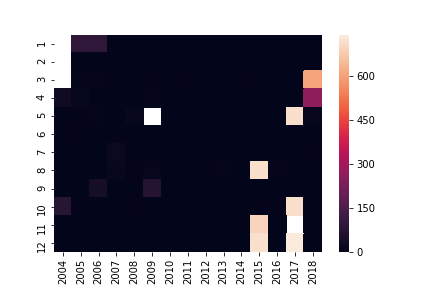
\includegraphics[scale = 0.6]{Chapter4_Results/figurs/heat_map_missing_values.png}
    \caption[Heatmap showing missing hours for all months or years.]{Heatmap displaying missing hours separated in month and years.}
    \label{fig:heatmap_missing_values}
\end{figure}

\subsection{Statistics}
Add some interesting statistics. Correlation maps, and matrices.
\textbf{I intend to compute som statistics for land and ocean, if only to include the code I've used to compute the land, sea, coastline masks.}

% Finished regriddidng files.
\subsection{Summarise the dataset ECC.}
Fractional cloud cover is computed from the cloud mask product retrieved by the second generations METeosat satellites. You can read more about this data in section \ref{sec:meteosat}. For simplicity we will refer to this dataset as European Cloud Cover Dataset, ECC from now on. The visual comparison between raw satellite images and cloud amount seem to agree. The cloud fractional distribution also retain the same shape as ERA5 and MODIS 6.1 Terra in the period from 2004 to 2018. \textbf{kilde?}

\subsubsection{Licences and Downloading Data} \label{sec:downloading_data}
Scripts for downloading the ERA5 data used in this thesis is available in the project GitHub on \href{https://github.com/hannasv/MS/tree/metos/downloading{\_}RA}{https://github.com/hannasv/MS/tree/metos/downloading{\_}RA}. However you will need to create a CDS-user. Follow the instructions on ECMWF homepages on \textit{how to download ERA5}. There are no scripts available for downloading METEOSAT data this is done using satellite retrievals at EUMETSATs Earth Observation Portal. Its freely available in hourly resolution. Scientist can apply for increased resolution up to 15min. Choose the cloud mask product in grb-format. By running \textbf{X - legg inn filnavn} you can generate your own files for regridding. The supplementary material only include the domain used in this thesis, because of GitHub has a maximum limit allowed for uploading. 

\section{AR models}

\section{Experiments}






